\documentclass[../main/main.tex]{subfiles}

% Put everything that shall appear in the results
% inside this document environment.
\begin{document}
In the following we present several plots showing the results of our experiment evaluations, starting with some information about our demographic data, before displaying general averaged results, followed by a demonstration of individual evaluations of the task performance and bier scores.
\subsection{Demographic Data}
Our questionnaire shown in \ref{appendix:questionaire} has been evaluated on 14 subjects. Their average age was 31.5 years within a range of our youngest 22 year old subject and our oldest subject of 62 years. The group consisted of 6 females and 8 males, all with german nationality and german as their mother language. Their professions included one computer scientist, one scientific coworker, one social worker, one curative educator, one insurance agent and nine students. The subjects of the later included \textit{Psychology in IT} 5 times and \textit{Computer Science} two times. One student's subject was \textit{Social Works}, one was studying \textit{Psychology} and one student came from the field of \textit{Cognitive Science}.
\subsection{Averaged Task Performance and Brier Score}
The average task performance of our subjects is shown in \ref{fig:avg_scores}, with an absolute mean of [TODO: X], averaged across all subjects and tasks. 
\begin{figure}[h]
	\centering
	\captionsetup{justification=centering}
	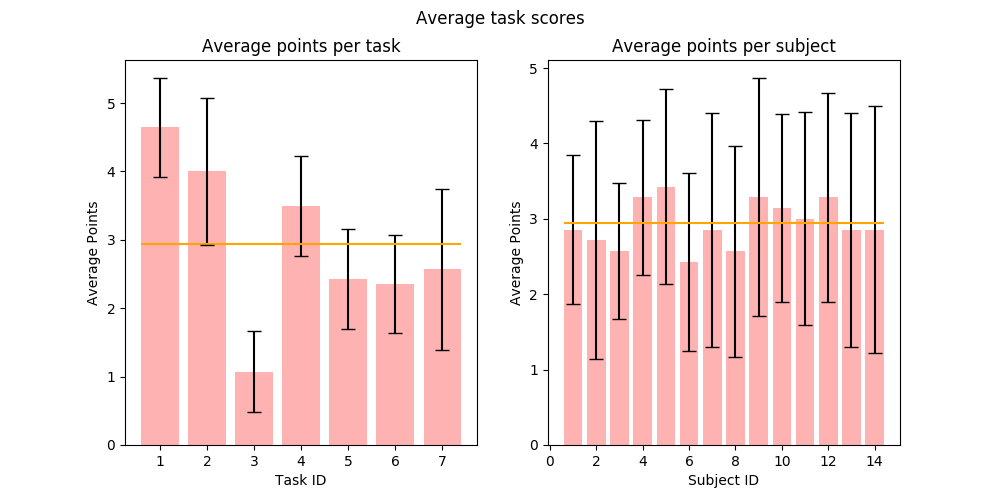
\includegraphics[width=\textwidth]{../assets/average_task_scores.png}
	\caption{Means and standard deviations of the achieved task scores, averaged over subjects in the left and over tasks in the right plot. The orange line displays the overall mean of [TODO], averaged over both variables.]}
	\label{fig:avg_scores}
\end{figure}
The subjects abilities to judge about their own performance, encode by the average brier score, is displayed in figure \ref{fig:avg_brier} with an overall average of 0.14. 
\begin{figure}[h]
	\centering
	\captionsetup{justification=centering}
	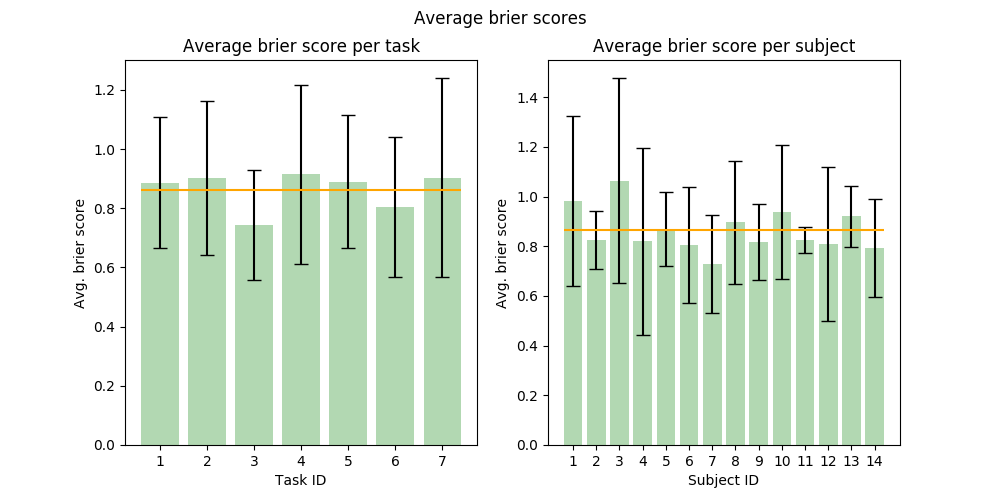
\includegraphics[width=\textwidth]{../assets/average_brier_scores.png}
	\caption{Means and standard deviations of the calculated brier scores, averaged over subjects in the left and over tasks in the right plot. The orange line displays the overall mean of 0.14, averaged over both variables.}
	\label{fig:avg_brier} 
\end{figure}
Please note that we excluded the 8th task from our questionnaire in figure \ref{appendix:questionaire}. For interpretation of these values, please refer to our discussion of the experiment in section \ref{sec:discussion}.
\subsection{Individual Evaluations}
We did individual evaluations of our subjects' task performance, brier scores and confidence ratings. While all figures can be found in appendix \ref{appendix:individual_evaluations}, figure \ref{fig:erhn_results} displays an example for one subject.
\begin{figure}[h]
	\centering
	\captionsetup{justification=centering}
	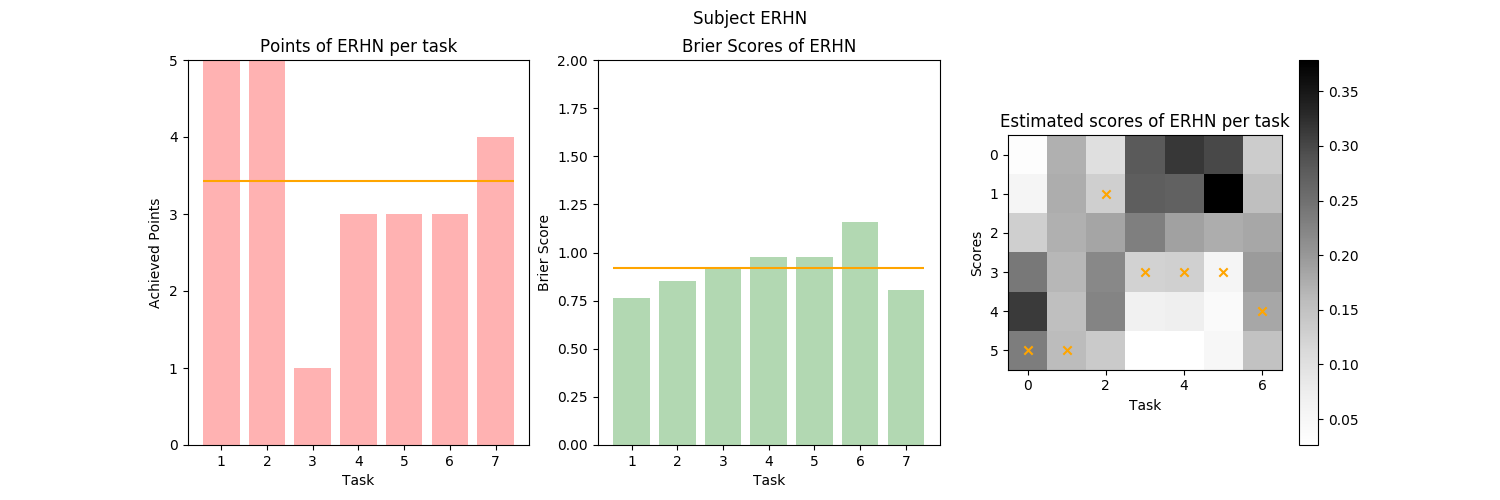
\includegraphics[width=\textwidth]{../assets/ERHN_results.png}
	\caption{Example graphic of our individual evaluations for subject \textit{ERHN}. We again plotted the achieved discrete scores per task on the left and the calculated brier-scores per task in the middle. The orange line displays the mean values for both bar plots, averaged over all tasks. The subject's estimated discrete probabilities of achieving a score are shown in the right graphic, where the orange x marks the actual achieved score in the task. [TODO: FIX X-RANGE OF RIGHT PLOT!]. One could already conclude a tendency of this subject to give underconfident ratings.}
	\label{fig:erhn_results} 
\end{figure}
\subsection{Overal Confidence}
\subsection{Task performance vs Brier Score}
\subsection{Calibrations}
\end{document}